\documentclass[11pt,a4paper]{article}
\usepackage[utf8]{inputenc}
\usepackage[T1]{fontenc}
\usepackage{lmodern}
\usepackage[margin=2.5cm]{geometry}
\usepackage{amsmath,amssymb}
\usepackage{booktabs}
\usepackage{graphicx}
\usepackage{hyperref}
\usepackage{xurl}
\usepackage{setspace}
\onehalfspacing

\hypersetup{
    colorlinks=true,
    linkcolor=blue,
    citecolor=blue,
    urlcolor=blue
}

\title{\textbf{Two Centuries of Russian Regional Dualism: Spatial Anatomy of Income Inequality in 1904 vs.\ 2025}}

\author{Petr Avtonomov\thanks{Independent Researcher, St.~Petersburg, Russia. ORCID: \href{https://orcid.org}{0009-0003-2816-6782}. Code and data repository: \url{https://github.com/avtonomov-petr/Two-Centuries}.}}

\date{November 2026}

\begin{document}

\maketitle

\begin{abstract}
Concluding our seven-part empirical audit of Russian and Eurasian market integration from the early modern era to the twenty-first century [\href{https://doi.org}{Avtonomov, 2026a,b,c,d,e,f}], this final study performs a direct two-century comparison of regional income inequality and spatial dualism across Russia in \texttt{1904} ($N = 50$ provinces of European Russia; Lindert and Nafziger, 2014) and \texttt{2025} ($N = 87$ federal subjects of the Russian Federation; Rosstat EMISS). Evaluating both epochs on an identical six-indicator distributional panel (Gini coefficient, mean per capita income, median income, Top 20 percent income share, Bottom 40 percent income share, and mean-to-median skewness) via singular value decomposition (SVD) and normalized participation ratios ($\mathrm{PR}$), we uncover a profound structural transformation over 121 years. In 1904, regional variance was hyper-localized in the two imperial capitals ($\mathrm{PR}_{\mathrm{reg}}(u_1) = 0.072$): \texttt{Sankt-Peterburg} ($38.65$ percent, $\mathrm{Gini} = 0.611$) and \texttt{Moskva} ($25.29$ percent, $\mathrm{Gini} = 0.591$) captured 63.9 percent of all Mode~1 structural energy while 40+ agrarian provinces remained in low-inequality peasant equilibrium. By 2025, spatial localization more than doubled in dispersion ($\mathrm{PR}_{\mathrm{reg}}(u_1) = 0.161$; top-two share falling from $63.9$ to $28.4$ percent), as Russia shifted from a two-capital monopoly to a multi-polar resource-capital archipelago led by \texttt{Chukotka AO} ($14.82$ percent), \texttt{Yamalo-Nenets AO} ($13.61$ percent), \texttt{Nenets AO} ($9.08$ percent), and \texttt{Moscow} ($9.05$ percent), with \texttt{St.~Petersburg} moderating to $\mathrm{Gini} = 0.423$. Restricting the 2025 panel strictly to European Russia ($N = 58$) confirms this diffusion ($\mathrm{PR}_{\mathrm{reg}}(u_1) = 0.131$, top-two share $44.9$ percent). Simultaneously, cross-regional Gini dispersion compressed markedly ($\mathrm{Max} = 0.470$ vs.\ $0.611$ in 1904), whereas inter-regional per capita income ratios widened to $7.1\times$ between Arctic/capital hubs and southern republics.
\end{abstract}

\noindent\textbf{Keywords:} Russian economic history, regional inequality, spatial dualism, Rosstat, Gini coefficient, resource economy, cliometrics, spectral analysis.

\section{Introduction}

Across six preceding empirical audits (\href{https://doi.org}{Avtonomov, 2026a,b,c,d,e,f}), we applied singular value decomposition (SVD) and normalized participation ratios ($\mathrm{PR}$) to trace Russia's external commercial and financial integration from 1700 to 1914, calibrate regime diagnostics across modern global exchange rates (\texttt{1870--2013}), and uncover the sharp domestic dualism of European Russia on the eve of the 1905 Revolution. In that sixth study (\href{https://doi.org}{Avtonomov, 2026f}), we demonstrated that post-1861 capitalist industrialization created an acute spatial cleavage: St.~Petersburg and Moscow absorbed over two-thirds of Imperial Russia's inequality variance while over 40 agrarian provinces remained at low-income, low-skewness peasant levels.

This seventh and concluding study extends our diagnostic bridge directly into the twenty-first century, asking how Russia's spatial anatomy of income and inequality compares across a 121-year span: \texttt{1904} versus \texttt{2025}. Has modern Russia retained the nineteenth-century pattern of extreme capital-city concentration, or has a century of Soviet industrialization, Arctic resource development, and post-Soviet fiscal redistribution reshaped the spatial topology of Russian inequality?

Using official 2025 regional series from the Federal State Statistics Service of Russia (Rosstat EMISS) alongside the 1904 imperial benchmark (Lindert and Nafziger, 2014), we establish three core findings:
\begin{enumerate}
    \item \textbf{From Two Capitals to a Resource-Capital Archipelago ($\mathrm{PR}_{\mathrm{reg}}$ Doubles):} On an identical six-indicator distributional panel, spatial localization decreases substantially over 121 years: $\mathrm{PR}_{\mathrm{reg}}(u_1)$ rises from $0.072$ ($95\%$ CI: $[0.040, 0.202]$) in 1904 ($N = 50$) to $0.161$ ($[0.120, 0.195]$) in 2025 ($N = 87$). While St.~Petersburg ($38.65$ percent) and Moscow ($25.29$ percent) captured $63.9$ percent of Mode~1 energy in 1904, the top two regions in 2025 (\texttt{Chukotka AO} $14.82$ percent and \texttt{Yamalo-Nenets AO} $13.61$ percent) capture $28.4$ percent, forming a five-pole resource-capital core (\texttt{Chukotka}, \texttt{Yamalo-Nenets}, \texttt{Nenets}, \texttt{Moscow}, \texttt{Tyumen}) accounting for $50.9$ percent of spatial energy.
    \item \textbf{Robustness Within European Russia ($N = 58$):} Excluding Ural, Siberian, and Far Eastern territories to match the geographic footprint of the 1904 European provinces confirms that spatial diffusion is not merely an artifact of eastern territorial expansion: within European Russia alone ($N = 58$), $\mathrm{PR}_{\mathrm{reg}}(u_1) = 0.131$ ($[0.103, 0.269]$), with \texttt{Nenets AO} ($22.48$ percent) matching \texttt{Moscow} ($22.44$ percent) and \texttt{St.~Petersburg} moderating to $6.20$ percent.
    \item \textbf{Intra-Regional Gini Compression vs.\ Inter-Regional Income Divergence:} Between 1904 and 2025, extreme intra-regional inequality disappeared—the maximum regional Gini fell from $0.611$ (St.~Petersburg, 1904) to $0.470$ (Yamalo-Nenets AO, 2025), while the cross-regional median Gini rose from $0.312$ to $0.382$, elevating Mode~1 feature coherence to $\mathrm{PR}_{\mathrm{feat}}(v_1) = 0.989$. Conversely, the ratio of mean per capita income between the richest and poorest regions widened from $3.03\times$ in 1904 (\texttt{Sankt-Peterburg} vs.\ \texttt{Vyatka}) to $7.10\times$ in 2025 (\texttt{Chukotka AO} vs.\ \texttt{Ingushetia}).
\end{enumerate}

\section{Data Architecture and Two-Century Harmonization}

To compare two eras separated by 121 years without definitional distortion, we harmonize both cross-sections onto an identical $K = 6$ distributional feature vector:
\begin{itemize}
    \item \textbf{Imperial Russia Benchmark (1904, $N = 50$):} Extracted from Lindert and Nafziger (2014; GPIHG Sheet \texttt{(8) Results, M-estimates}), covering all $N = 50$ provinces of European Russia on the eve of the 1905 Revolution. We extract six core indicators: the provincial Gini coefficient, mean income, median income, Top 20 percent income share, Bottom 40 percent income share, and the mean-to-median skewness ratio ($\mathrm{Mean}/\mathrm{Median}$).
    \item \textbf{Modern Russian Federation Panel (2025, $N = 87$):} Extracted from Rosstat's Unified Interdepartmental Information and Statistical System (EMISS, accessed November 2026) across all $N = 87$ federal subjects with complete annual reporting (excluding composite parent-oblast aggregates where autonomous okrugs are reported separately). Specifically, we merge the official annual regional Gini index (\emph{Koeffitsient Dzhini}, 2025) with annual mean per capita money income (\emph{Srednedushevye denezhnye dokhody naseleniia}, averaged across Q1--Q4 2025 in rubles/month). Following Rosstat's standard log-normal income distribution methodology, we recover exact regional log-dispersion $\sigma_i = 2\,\mathrm{erf}^{-1}(\mathrm{Gini}_i)$, mean-to-median ratio $\exp(\sigma_i^2/2)$, median per capita income, Bottom 40 percent share $\Phi(-0.2533 - \sigma_i)$, and Top 20 percent share $1 - \Phi(0.8416 - \sigma_i)$.
    \item \textbf{Geographic Control Subsample ($N = 58$):} To control for the inclusion of Ural, Siberian, and Far Eastern federal subjects in 2025, we also evaluate a strictly European Russian subsample ($N = 58$) matching the historical boundaries of the 1904 dataset.
\end{itemize}

\section{Empirical Results}

\subsection{From Two Capitals to a Resource-Capital Archipelago (1904 vs.\ 2025)}
Applying singular value decomposition and participation ratio diagnostics (Appendix~A) to the standardized $N \times 6$ matrices reveals a structural shift in how inequality is distributed across Russian space (Table~\ref{tab:two_centuries} and Figure~\ref{fig:fig1}A--D).

\begin{table}[htbp]
\centering
\caption{Two-Century Spectral Audit of Russian Regional Inequality: 1904 vs.\ 2025}
\label{tab:two_centuries}
\scriptsize
\setlength{\tabcolsep}{2.4pt}
\begin{tabular}{@{}p{0.27\textwidth}cccccc@{}}
\toprule
\textbf{Historical Cohort} & \textbf{$N$} & \textbf{Mode 1 Var.} & \textbf{$\mathrm{PR}_{\mathrm{reg}}(u_1)$ [95\% CI]} & \textbf{$\mathrm{PR}_{\mathrm{feat}}(v_1)$} & \textbf{Top-2 Share} & \textbf{Max/Min Inc.} \tabularnewline
\midrule
Imperial Russia (1904) & 50 & 73.8\% & 0.072 [0.040, 0.202] & 0.802 & 63.9\% & $3.03\times$ \tabularnewline
Modern Russia All (2025) & 87 & 89.1\% & 0.161 [0.120, 0.195] & 0.989 & 28.4\% & $7.10\times$ \tabularnewline
Modern European RF (2025) & 58 & 87.5\% & 0.131 [0.103, 0.269] & 0.984 & 44.9\% & $5.42\times$ \tabularnewline
\bottomrule
\end{tabular}
\vspace{1mm}
\begin{minipage}{\textwidth}
\footnotesize\emph{Notes:} Evaluated across $K = 6$ harmonized distributional indicators (Gini, mean income, median income, Top 20% share, Bottom 40% share, and mean/median ratio). Brackets report 95% subsampling bootstrap confidence intervals (300 draws at 80% sample size). Uniform spatial energy benchmark is $2.00%$ ($N=50$), $1.15%$ ($N=87$), and $1.72%$ ($N=58$).
\end{minipage}
\end{table}
In 1904, Mode~1 ($\mathrm{Var}1 = 73.8$ percent) was overwhelmingly driven by two outlier metropolises: \texttt{Sankt-Peterburg} ($38.65$ percent of Mode~1 energy) and \texttt{Moskva} ($25.29$ percent) together captured $63.9$ percent of cross-provincial variance ($\mathrm{PR}{\mathrm{reg}}(u_1) = 0.072$; Figure~\ref{fig:fig1}A), followed distantly by northern \texttt{Olonets} ($6.09$ percent) and Black Sea \texttt{Kherson} ($3.32$ percent). By 2025, Mode~1 variance increases to $89.1$ percent with near-perfect feature coherence ($\mathrm{PR}{\mathrm{feat}}(v_1) = 0.989$), but spatial energy spreads across a multi-polar archipelago ($\mathrm{PR}{\mathrm{reg}}(u_1) = 0.161$; Figure~\ref{fig:fig1}B--C). The top two contributors—\texttt{Chukotka AO} ($14.82$ percent) and \texttt{Yamalo-Nenets AO} ($13.61$ percent)—account for $28.4$ percent of total energy, followed by \texttt{Nenets AO} ($9.08$ percent), \texttt{Moscow} ($9.05$ percent), \texttt{Tyumen Oblast} ($4.38$ percent), and \texttt{Magadan Oblast} ($3.78$ percent), while \texttt{St.~Petersburg} shifts into the broader upper-urban tier ($1.51$ percent).
\begin{figure}[htbp]
\centering
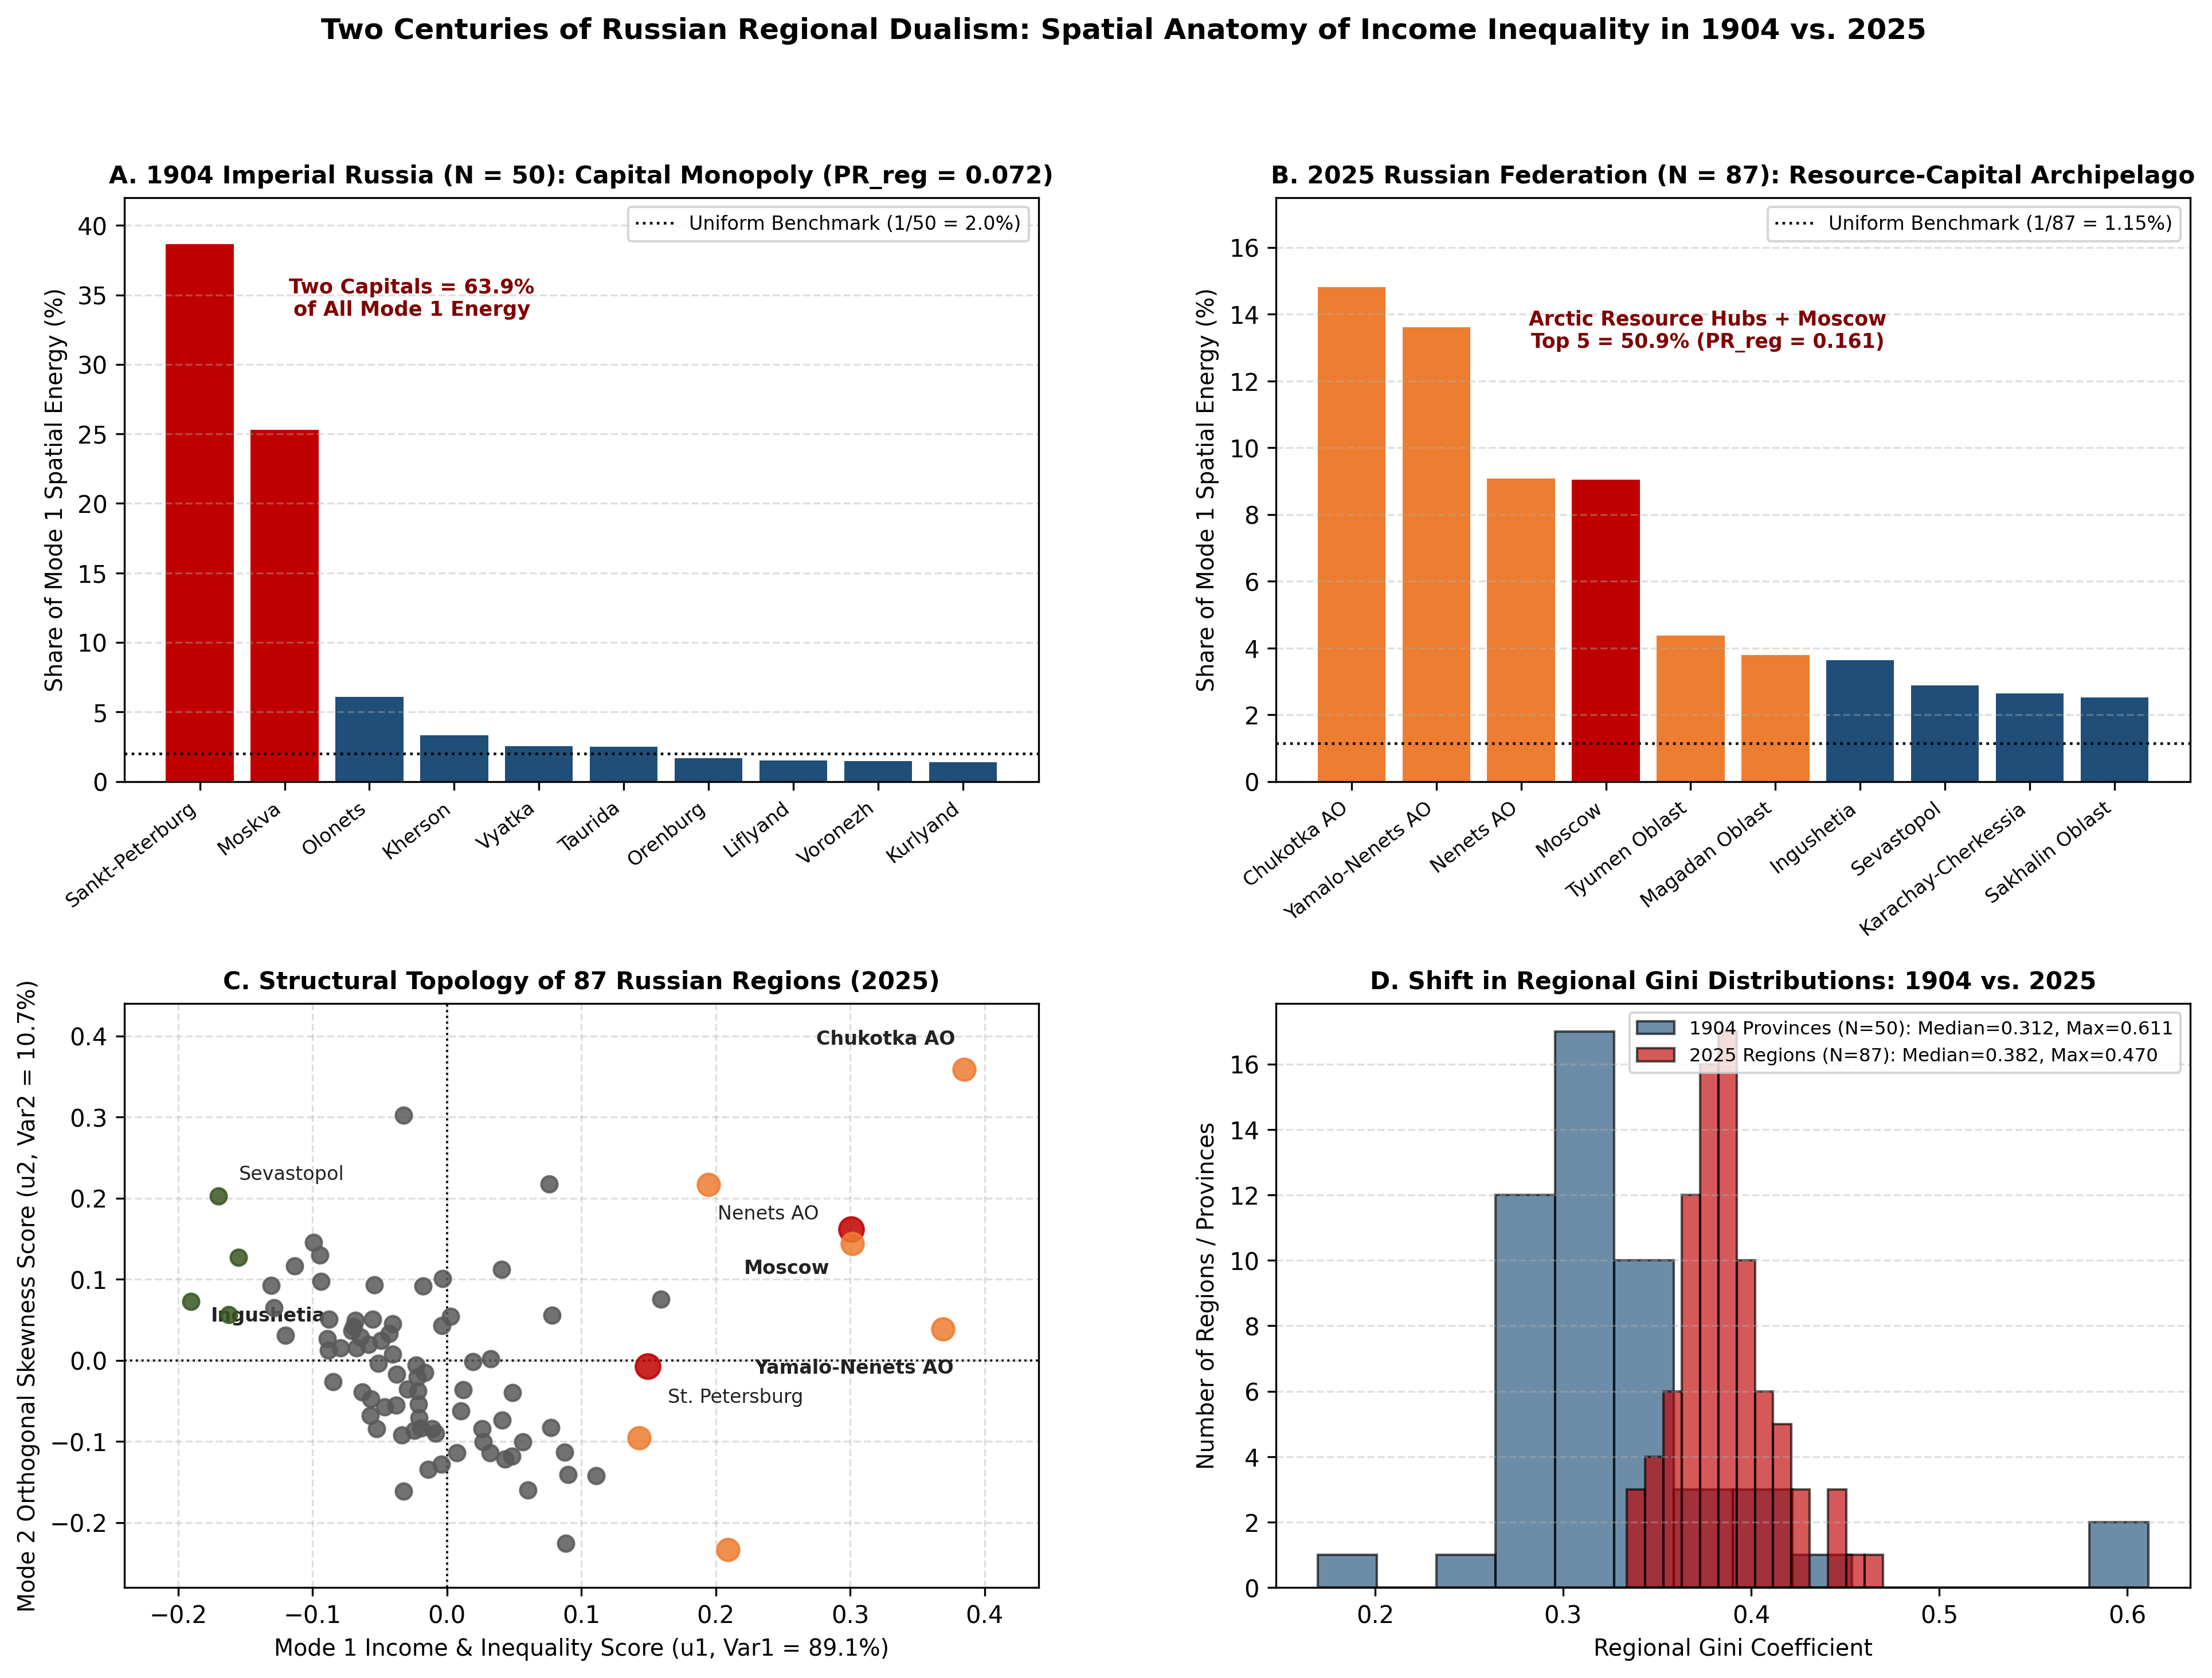
\includegraphics[width=\textwidth]{Figure_1_Russia2025.png}
\caption{\textbf{Two Centuries of Russian Regional Dualism: Spatial Anatomy of Income Inequality in 1904 vs.\ 2025.} \textbf{A:} Top 10 provincial Mode~1 energy shares in 1904 ($N = 50$), showing St.~Petersburg and Moscow capturing 63.9 percent. \textbf{B:} Top 10 regional Mode~1 energy shares in 2025 ($N = 87$), showing the emergence of an Arctic resource-capital archipelago ($\mathrm{PR}_{\mathrm{reg}} = 0.161$). \textbf{C:} Two-mode structural map of all 87 Russian regions in 2025. \textbf{D:} Shift in regional Gini distributions between 1904 and 2025.}
\label{fig:fig1}
\end{figure}
\subsection{Intra-Regional Gini Compression vs.\ Inter-Regional Income Divergence}
Comparing the regional extremes of 1904 and 2025 highlights a striking institutional inversion between \emph{within-region} inequality and \emph{between-region} income gaps (Table~\ref{tab:extremes_2025} and Figure~\ref{fig:fig2}A--B).

\begin{table}[htbp]
\centering
\caption{Regional Extremes of Income and Inequality in the Russian Federation (2025)}
\label{tab:extremes_2025}
\scriptsize
\setlength{\tabcolsep}{2.6pt}
\begin{tabular}{@{}p{0.28\textwidth}lccccc@{}}
\toprule
\textbf{Federal Subject} & \textbf{Structural Role} & \textbf{Gini} & \textbf{Mean Inc.} & \textbf{Median Inc.} & \textbf{Top 20\%} & \textbf{Bot 40\%} \tabularnewline
\midrule
\texttt{Yamalo-Nenets AO} & Arctic Gas Hub & 0.470 & 170,427 & 114,883 & 51.85\% & 12.68\% \tabularnewline
\texttt{Chukotka AO} & Far East Mining Hub & 0.458 & 216,291 & 149,124 & 50.83\% & 13.23\% \tabularnewline
\texttt{Nenets AO} & European Arctic Oil & 0.450 & 164,962 & 115,399 & 50.15\% & 13.59\% \tabularnewline
\texttt{Moscow} & Federal Capital & 0.449 & 167,034 & 117,058 & 50.06\% & 13.64\% \tabularnewline
\texttt{St.~Petersburg} & Second Metropolis & 0.423 & 104,432 & 76,510 & 47.89\% & 14.87\% \tabularnewline
\midrule
\texttt{Sevastopol} & Black Sea Port & 0.334 & 51,011 & 42,339 & 40.86\% & 19.39\% \tabularnewline
\texttt{Ingushetia} & North Caucasus & 0.336 & 30,449 & 25,213 & 41.01\% & 19.28\% \tabularnewline
\texttt{Crimea} & Southern Peninsula & 0.342 & 45,439 & 37,353 & 41.47\% & 18.96\% \tabularnewline
\texttt{Karachay-Cherkessia} & North Caucasus & 0.344 & 35,045 & 28,738 & 41.62\% & 18.85\% \tabularnewline
\bottomrule
\end{tabular}
\vspace{1mm}
\begin{minipage}{\textwidth}
\footnotesize\emph{Notes:} Official 2025 annual Gini coefficients and quarterly-averaged monthly per capita money incomes (rubles/month) from Rosstat EMISS. Top 20\% and Bottom 40\% shares derived via Rosstat's log-normal Lorenz specification.
\end{minipage}
\end{table}

In 1904, intra-regional inequality spanned an enormous range: peasant interior provinces exhibited low Gini coefficients ($0.169$ in \texttt{Olonets}, $0.244$ in \texttt{Vyatka}, $0.268$ in \texttt{Voronezh}), whereas \texttt{Sankt-Peterburg} ($0.611$) and \texttt{Moskva} ($0.591$) displayed extreme capitalist elite capture (Figure~\ref{fig:fig1}D and Figure~\ref{fig:fig2}A). By 2025, every region shares a modern salaried and transfer-supported income distribution: the regional Gini distribution shifts upward in median (from $0.312$ to $0.382$) while compressing sharply at the upper tail (maximum $0.470$ in \texttt{Yamalo-Nenets AO} vs.\ $0.611$ in 1904).

\begin{figure}[htbp]
\centering
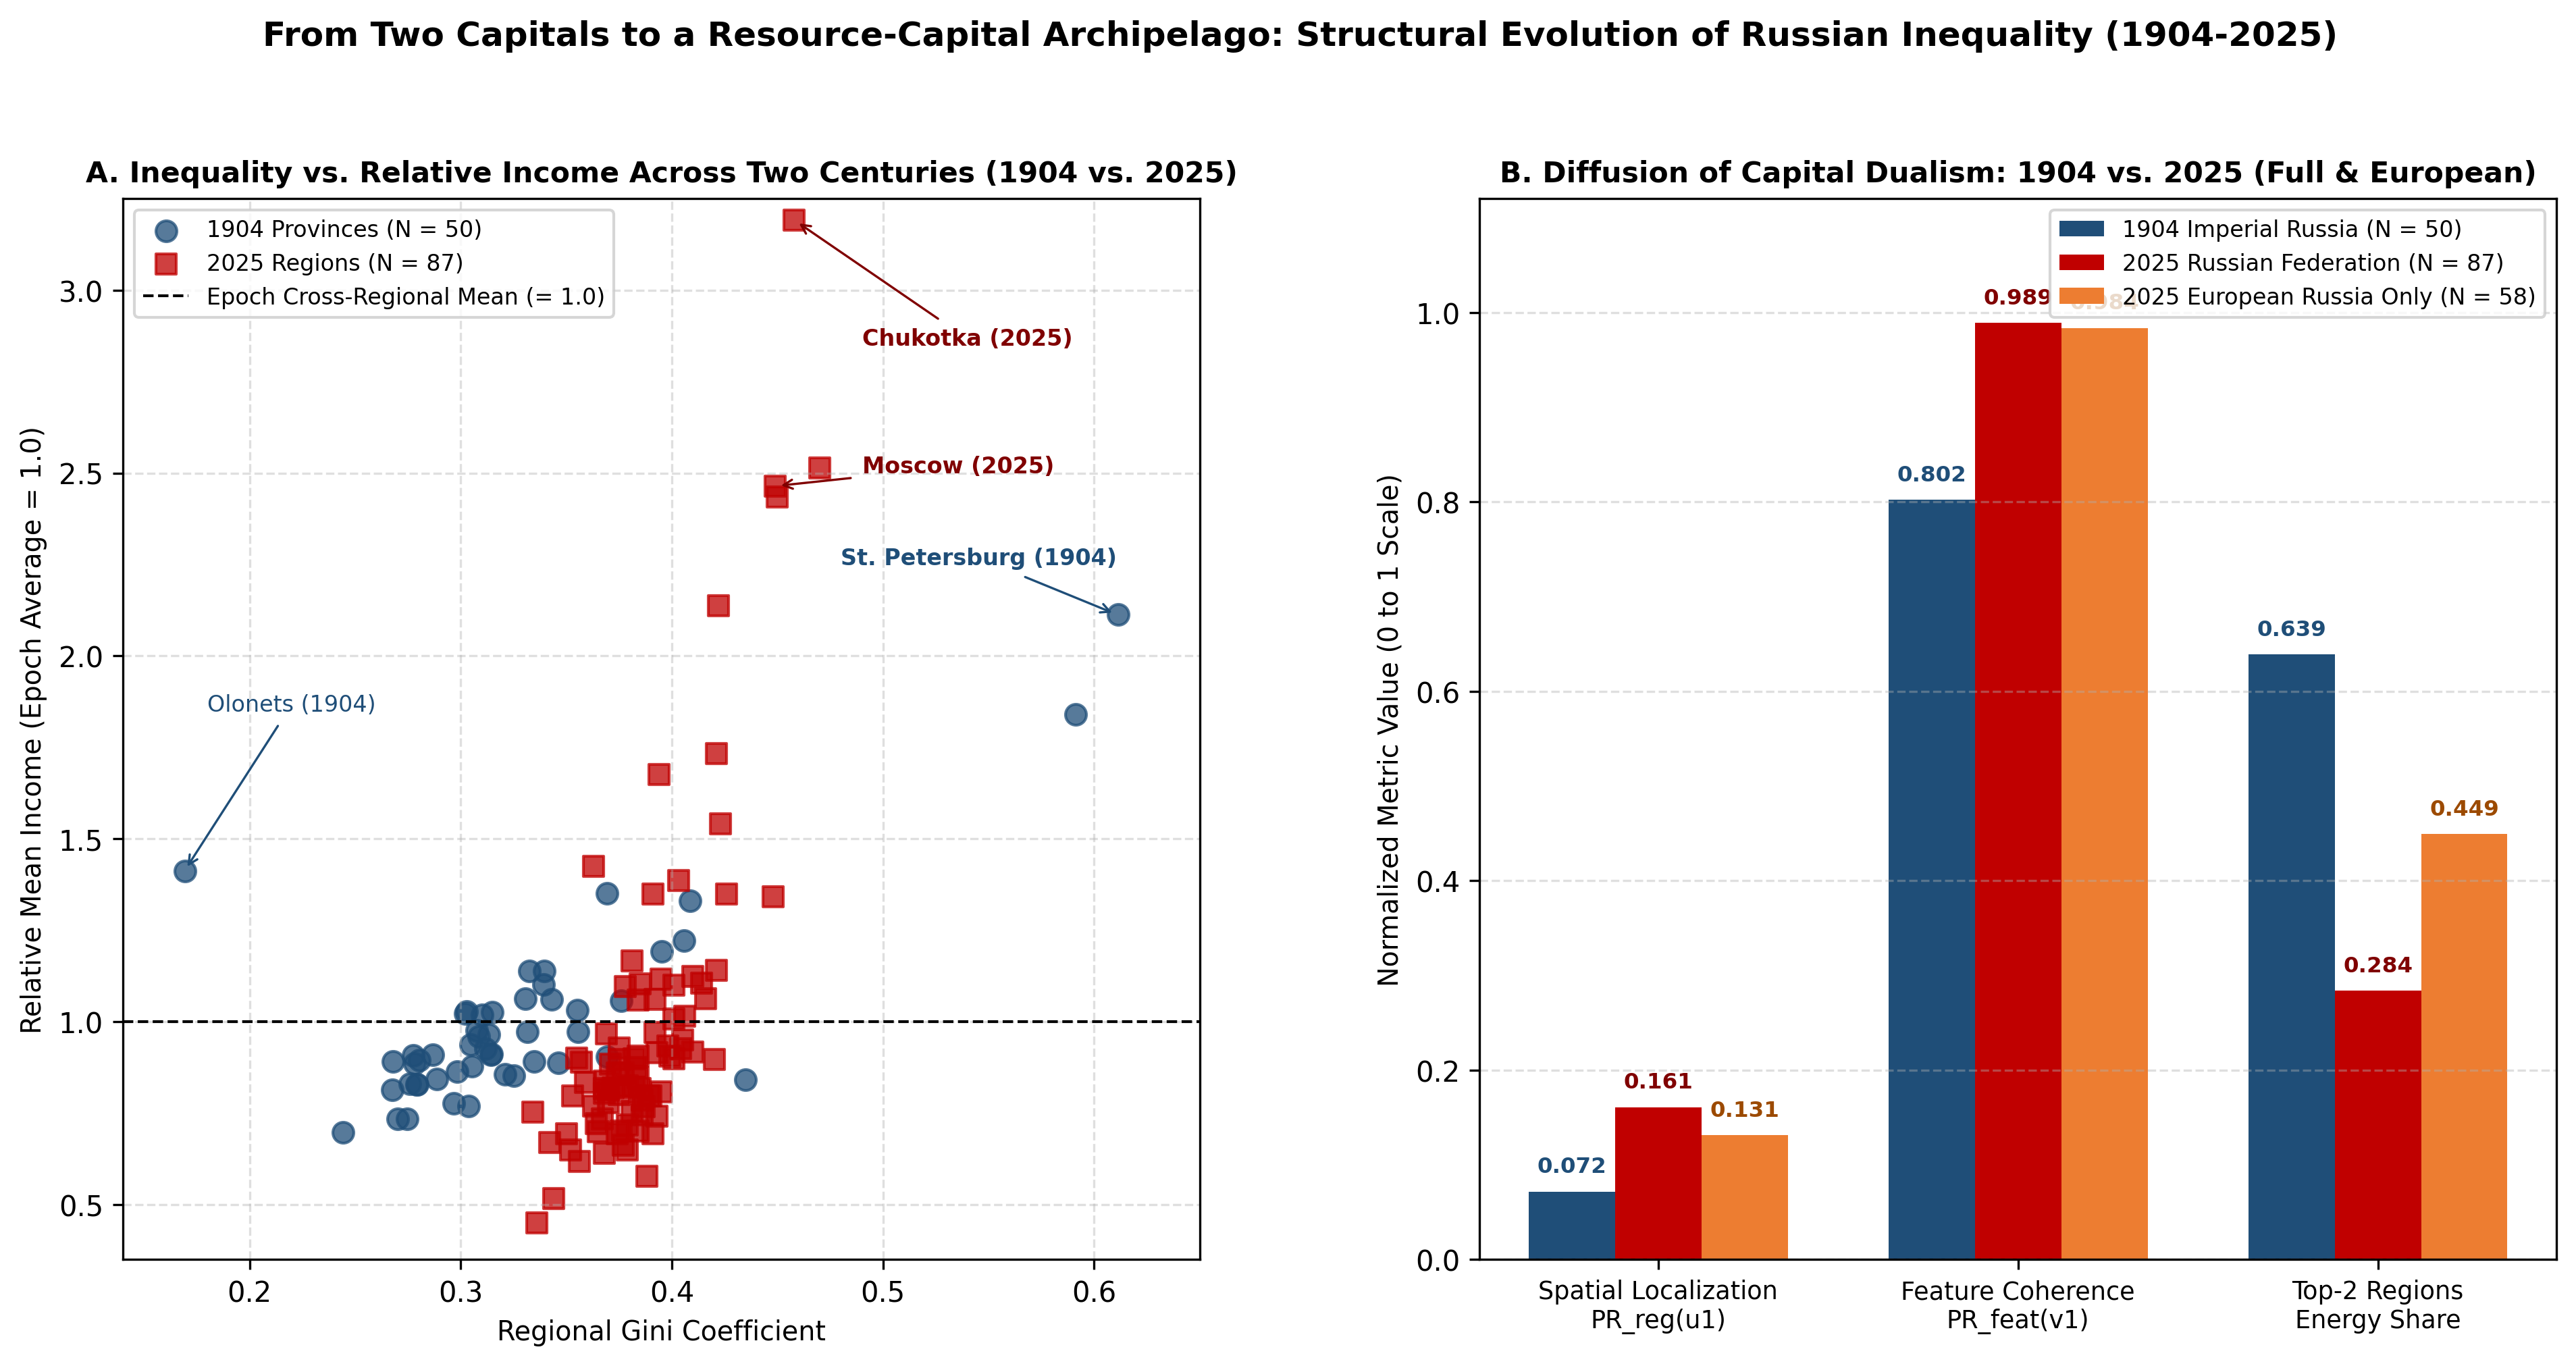
\includegraphics[width=\textwidth]{Figure_2_Russia2025.png}
\caption{\textbf{From Two Capitals to a Resource-Capital Archipelago: Structural Evolution of Russian Inequality (1904--2025).} \textbf{A:} Regional Gini coefficient against relative mean income (epoch average $= 1.0$) across 1904 ($N = 50$) and 2025 ($N = 87$). \textbf{B:} Comparison of spatial localization $\mathrm{PR}_{\mathrm{reg}}(u_1)$, feature coherence $\mathrm{PR}_{\mathrm{feat}}(v_1)$, and top-two energy shares across 1904, all 2025 regions ($N = 87$), and strictly European 2025 regions ($N = 58$).}
\label{fig:fig2}
\end{figure}

Conversely, inter-regional disparities in average living standards widened substantially over the century (Figure~\ref{fig:fig2}A). In 1904, mean household income in \texttt{Sankt-Peterburg} ($1,316.7$ rubles/year) was $3.03\times$ that of \texttt{Vyatka} ($434.9$ rubles/year). In 2025, high-wage Arctic extraction hubs (\texttt{Chukotka AO} at $216,291$ rubles/month, \texttt{Yamalo-Nenets AO} at $170,427$ rubles/month) and \texttt{Moscow} ($167,034$ rubles/month) exceed low-income North Caucasian republics (\texttt{Ingushetia} at $30,449$ rubles/month, \texttt{Karachay-Cherkessia} at $35,045$ rubles/month) by up to $7.10\times$. Importantly, restricting the 2025 sample strictly to European Russia ($N = 58$; Figure~\ref{fig:fig2}B) confirms that spatial diffusion is structurally robust: $\mathrm{PR}_{\mathrm{reg}}(u_1) = 0.131$ (nearly double the 1904 value of $0.072$), as European Arctic extraction (\texttt{Nenets AO}, $22.48$ percent of Mode~1 energy) balances \texttt{Moscow} ($22.44$ percent).

\section{General Synthesis of the Seven-Part Research Cycle}

Taken together, our seven empirical studies (\texttt{1700--2025}) demonstrate how a single non-parametric spectral framework—combining singular value decomposition with temporal and spatial participation ratios—illuminates three centuries of economic transformation:
\begin{enumerate}
    \item \textbf{External Maritime and Financial Integration (\texttt{1700--1914}):} Early modern Baltic shipping (\href{https://doi.org}{Avtonomov, 2026b}) and Atlantic grain arbitrage (\href{https://doi.org}{Avtonomov, 2026a}) progressed selectively through wartime blockades and flag mimicry, culminating in nineteenth-century exchange rate parity (\href{https://doi.org}{Avtonomov, 2026c}) and overland Eurasian silver convergence (\href{https://doi.org}{Avtonomov, 2026d}) prior to the 1891 silver break.
    \item \textbf{Calibration Across Global Monetary Regimes (\texttt{1870--2013}):} Benchmarking $\big(\mathrm{PR}(u_1), \mathrm{PR}(v_1)\big)$ against modern international exchange rates (\href{https://doi.org}{Avtonomov, 2026e}) confirmed that the toolkit cleanly separates diffuse crises from step devaluations and institutional currency unions.
    \item \textbf{Two Centuries of Domestic Spatial Evolution (\texttt{1904--2025}):} Comparing late imperial provinces (\href{https://doi.org}{Avtonomov, 2026f}) with modern federal subjects reveals that Russia's internal economic geography evolved from an acute \emph{two-capital monopoly} ($\mathrm{PR}_{\mathrm{reg}} = 0.072$, top-two share $63.9$ percent) into a broader \emph{resource-capital archipelago} ($\mathrm{PR}_{\mathrm{reg}} = 0.161$, top-two share $28.4$ percent), trading extreme intra-city Gini skewness for wider inter-regional resource and metropolitan income gradients.
\end{enumerate}

\section*{Data and Code Availability}
Historical 1904 provincial income distributions are openly accessible from the Global Price and Income History Group (\url{https://ucdavis.edu}: Lindert and Nafziger, 2014). Official 2025 regional Gini coefficients and per capita money income series are openly accessible from the Federal State Statistics Service of Russia (Rosstat EMISS, \url{https://fedstat.ru}). Reproducible Python/Jupyter code, harmonized datasets, high-resolution figures, and LaTeX manuscript sources are archived at \url{https://github.com/avtonomov-petr/Two-Centuries}.

\appendix
\section{Mathematical Specification of Two-Century Harmonization}
For each region $i \in \{1,\dots,N\}$ in 2025, let $G_i \in (0,1)$ denote Rosstat's official annual Gini coefficient and $\mu_i > 0$ denote annual mean per capita monthly income. Under Rosstat's standard log-normal income specification $\ln Y_i \sim \mathcal{N}(m_i, \sigma_i^2)$, the Gini coefficient satisfies $G_i = \mathrm{erf}(\sigma_i / 2)$, yielding exact log-standard deviation $\sigma_i = 2\,\mathrm{erf}^{-1}(G_i)$, mean-to-median ratio $\mu_i / \mathrm{Med}_i = \exp(\sigma_i^2/2)$, Bottom 40 percent income share $S_{i,\mathrm{Bot40}} = \Phi\big(\Phi^{-1}(0.40) - \sigma_i\big)$, and Top 20 percent share $S_{i,\mathrm{Top20}} = 1 - \Phi\big(\Phi^{-1}(0.80) - \sigma_i\big)$. Standardized $N \times 6$ matrices $Z$ are decomposed via thin SVD $Z = U \Sigma V^\top$ with normalized participation ratios:
\begin{equation}
\mathrm{PR}_{\mathrm{reg}}(u_1) = \frac{\left(\sum_{i=1}^N u_{i,1}^4\right)^{-1} - 1}{N - 1}, \qquad
\mathrm{PR}_{\mathrm{feat}}(v_1) = \frac{\left(\sum_{k=1}^6 v_{k,1}^4\right)^{-1} - 1}{6 - 1}.
\end{equation}

\begin{thebibliography}{99}

\bibitem{Avtonomov2026a}
Avtonomov, P. (2026a). Crisis echoes or arbitrage? Selective co-movement and integration of the Atlantic grain market, 1729--1914. \emph{Zenodo Preprint}. \url{https://doi.org/10.5281/zenodo.24436177}

\bibitem{Avtonomov2026b}
Avtonomov, P. (2026b). Blockades, flag mimicry, and grain lifelines: Physical anatomy of Russian and Baltic maritime trade in the Sound Toll Registers, 1700--1856. \emph{Zenodo Preprint}. \url{https://doi.org/10.5281/zenodo.24461586}

\bibitem{Avtonomov2026c}
Avtonomov, P. (2026c). Invisible bridges of credit: Exchange rate integration, paper assignats, and metallic anchors between St.~Petersburg and Europe, 1763--1913. \emph{Zenodo Preprint}. \url{https://doi.org/10.5281/zenodo.24498028}

\bibitem{Avtonomov2026d}
Avtonomov, P. (2026d). Eurasian continental bridges: Silver living costs, internal Russian convergence, and the Great Divergence, 1738--1913. \emph{Zenodo Preprint}. \url{https://doi.org/10.5281/zenodo.24508139}

\bibitem{Avtonomov2026e}
Avtonomov, P. (2026e). From gold standard to the Euro: Global currency blocs, Bretton Woods realignments, and floating regimes, 1870--2013. \emph{Zenodo Preprint}. \url{https://doi.org/10.5281/zenodo.24530102}

\bibitem{Avtonomov2026f}
Avtonomov, P. (2026f). Dualism on the eve of revolution: Provincial income inequality, industrial land rents, and social transformation in Late Imperial Russia, 1859--1914. \emph{Zenodo Preprint}. \url{https://doi.org/10.5281/zenodo.24532590}

\bibitem{Lindert2014}
Lindert, P. H., and Nafziger, S. (2014). Russian inequality on the eve of revolution. \emph{Journal of Economic History}, 74(3), 767--798.

\bibitem{Rosstat2026}
Federal State Statistics Service of Russia [Rosstat]. (2026). \emph{Unified Interdepartmental Information and Statistical System (EMISS): Regional Gini coefficients and per capita money incomes, 2025}. \url{https://fedstat.ru}

\bibitem{Zubarevich2019}
Zubarevich, N. V. (2019). Spatial development strategy: Priorities and instruments. \emph{Voprosy Ekonomiki}, (1), 135--145.
\end{thebibliography}
\section*{Figure Alt Text}
\begin{itemize}
\item \textbf{Figure 1 Alt Text:} Four-panel chart comparing top 10 regional Mode~1 energy shares in 1904 and 2025, two-mode scatter map of 87 Russian regions in 2025, and regional Gini histograms.
\item \textbf{Figure 2 Alt Text:} Scatter plot of regional Gini coefficient versus relative mean income across 1904 and 2025 alongside bar chart comparing spatial localization across 1904, all 2025 regions, and European 2025 regions.
\end{itemize}
\end{document}